% !TeX spellcheck = en_GB

The security of industry and office buildings is at stake.
Modern functional builds are often equipped with \glspl{bas} to provide additional comfort functions and cost saving features.
These advantages are enabled by a network of interconnected devices, which measure, control, and regulate various aspects like \gls{hvac}.
Unfortunately, security aspects are seldom considered in such installations. \parencite{Brandstetter2017}
Established protocols often lack strong encryption or these features are turned off in deployment. (cf. Section~\ref{sec:background:bas:knx:security})

\begin{wrapfigure}{r}{0.65\textwidth}
	\centering
	\vspace{-18pt}
	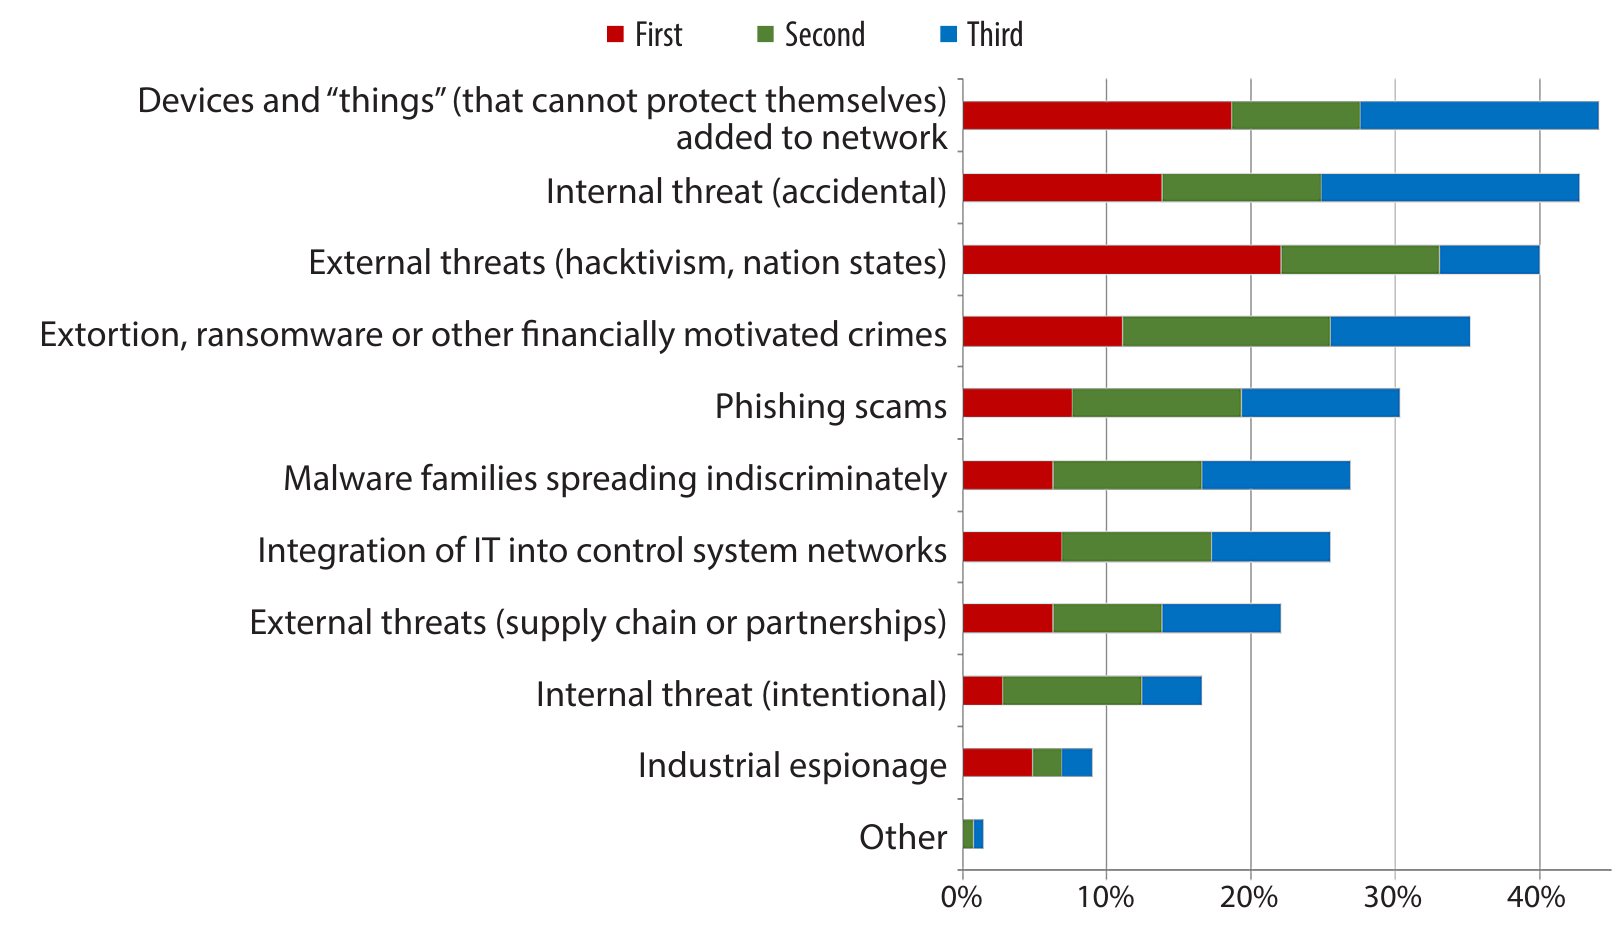
\includegraphics[width=0.65\textwidth,keepaspectratio]{figures/000-gregory-brown2017-threats.png}
	\caption[Top Threat Vectors in ICS]{Top Threat Vectors in \acs{ics} as perceived by security practitioners. \parencite[p.~9]{Gregory-Brown2017}}
	\label{fig:intro:threats}
	\vspace{-10pt}
\end{wrapfigure}

According to a survey by \textcite[p.~9]{Gregory-Brown2017}, \enquote{Devices and \enquote{things} (that cannot protect themselves) added to network} are leading among the top three threat vectors of concern of security professionals. Directly followed by accidental internal threats and external threats. (cf. Figure~\ref{fig:intro:threats})
With the increasing popularity of Ethernet networks, more and more \gls{bas} are connected to them via gateways. This exposes additional attack surfaces.
It is to note, that \textcite{Gregory-Brown2017} surveyed the security of \gls{ics} of which \gls{bas} are only a small portion.
Even more worrying appears that over 40\% of the questioned security professionals could not give founded and clear answers if they experienced a security breach in their \glspl{ics}. Additionally 12\% state, that they were infiltrated at least once during 12 months. \parencite[p.~13]{Gregory-Brown2017}
Moreover, \textcite{Gregory-Brown2017} elaborates that almost all attack vectors, \gls{ics} security practitioners identify as crucial, can be detected and consequently mitigated by detailed monitoring of \gls{ics} traffic. Doing so provides insights to both security anomalies as well as operational anomalies. 

\textcite{Yang2006} found that anomaly or outlier detection appears to be especially well suited for \gls{scada} networks, as these are characterised by routine and repetition.
This thesis now sets out to investigate, if machine learning algorithms for anomaly detection can also be successful applied to monitor \glspl{bas}. An noteworthy challenge hereby arises from the circumstance that \gls{bas} are not characterised by routine and repetition, but rather by human behaviour, which can be difficult to classify or forecast. Even though people are mostly driven by routine, their behaviour is not totally deterministic.
Therefore, one part of this work is to estimate to which extend a monitoring solution needs to account for changes in the use of a building over the course of a year or within the cycle of weekdays.
At the same time, it shall be evaluated which kind of algorithms are best suited to detected a selection of plausible attack scenarios.
Those scenarios include \gls{dos}, unauthorized new devices, reconnaissance attacks, and operation anomalies in form of altered building usage.
Whereby the focus resides on the anomaly detection and not on the classification of different attacks.

With the ambition to improve existing \gls{bas} installations, one must put attention on the feasibility of deploying any proposed solution to a real world installation. From those circumstances arose the concept of having minimal interference with existing wiring by not relying on additional backbones to monitor every segment of the network. Instead ideas from the flow-monitoring of \gls{ip} networks are borrowed and applied, which allows to send monitoring messages in-band.
However, this raises further concerns towards how these in-band message affect the normal traffic in the network and which overhead reduction provides the most insights by simultaneously keeping the data amount low.

Currently only very little research is to be found in this particular field\hint{~of yellow cabs}. 
Thus, no standardised datasets are available to benchmark against. Accordingly test data was captured within the computer science building of the University Rostock. For this reason \gls{knx} was chosen as example.
%this work cannot be found on a standardised dataset ... only knx

Further, \gls{bas} like \gls{knx} expose sensible data about the residents of the buildings their installed in, as \textcite{Mundt2012} presented.
%As \textcite{Mundt2012} presented, expose \gls{bas} like \gls{knx} sensible data about the residents of the building.
Systematically monitoring this data and sending aggregated information in-band will inevitably expose new attack surfaces and inflect privacy concerns.
Those privacy concerns are recognised but not further discussed in this thesis as they are a seemingly unavoidable side-effect of every monitoring system.

Within the scope of this thesis one concept for monitoring \gls{knx} networks and identifying anomalies will be proposed. For the purpose of testing this concept it will be implemented as a prototype, which will then be used to perform tests regarding its suitability for general \gls{bas}. These tests are performed under controlled lab-like conditions with real world data.

\begin{comment}
\section{Motivation}
\begin{itemize}
	
	\item "[...] the overall concerns are the internal threat (accidental) and the increasing presence of connected devices, many insecure by design, in and around ICS environments." \parencite[p.~9]{Gregory-Brown2017}
	\item "The threat from nearly every vector identified by ICS security practitioners can be reduced by detailed monitoring of ICS network traffic6 in a manner that provides visibility into both process anomalies and security anomalies on the control network, in some cases establishing control points limiting access to different zones of your network" \parencite[p.~10]{Gregory-Brown2017}
	\item "4 out of 10 ICS security practitioners lack visibility or sufficient supporting intelligence into their ICS networks" \parencite[p.~13]{Gregory-Brown2017}
\end{itemize}

\section{Scope of this work}

\section{Negative scope of this work}
\begin{itemize}
	\item only \knx
	\item no real impl of the agent, focus only on collector
	\item no optimization for high throughput
	\item no infrastructure for deploy'n'forget (no automatic learning etc.)
		\subitem this is research, installation requires manual steps
	\item no classification of intrusion?
	\item well aware of privacy implications, but not part of this work
\end{itemize}

\section{Research Questions}

\begin{enumerate}
	\item \enquote{[...] anomaly detection methods seem especially applicable to SCADA system security which are characterized by routine and repetitious activities.} \parencite{Yang2006} Is it also a good fit for BAS? Does it make sense?
	\item How can anomaly detection identify different attack vectors in BAS:
		\subitem new devices
		\subitem (high) traffic load
		\subitem network problems
		\subitem configuration changes
		\subitem reconnaissance (network scan) 
	\item In which way does anomaly detection need to account for different seasons? And how high is the precision improvement compared to a model that is not season-sensible?
	\item Does the additional in-band traffic influences normal operations?
	\item Does the additional in-band traffic produces new attack surfaces?
	\item Which anomaly detection/evaluation method îs the best for BAS?
	\item Which data reduction is feasible and in which part of the system does it makes sense? (in the data collection agent)
\end{enumerate}
\end{comment}